\documentclass[10pt,twocolumn]{article}

% use the oxycomps style file
\usepackage{oxycomps}

% usage: \fixme[comments describing issue]{text to be fixed}
% define \fixme as not doing anything special
\newcommand{\fixme}[2][]{#2}
% overwrite it so it shows up as red
\renewcommand{\fixme}[2][]{\textcolor{red}{#2}}
% overwrite it again so related text shows as footnotes
%\renewcommand{\fixme}[2][]{\textcolor{red}{#2\footnote{#1}}}

% read references.bib for the bibtex data
\bibliography{references.bib}

% include metadata in the generated pdf file
\pdfinfo{
    /Title (Common Vulnerabilities and Exposures Compilation Web App)
    /Author (Elise Corwin)
}

% set the title and author information
\title{Common Vulnerabilities and Exposures Compilation Web App}
\author{Elise Corwin}
\affiliation{Occidental College}
\email{ecorwin@oxy.edu}

\begin{document}

\maketitle

\section{Introduction and Problem Context}
Reflecting on my summer internship as a Cyber Security Analyst, I was interested in how cyber security employees discovered vulnerabilities given the dynamic and quickly changing cyber threat landscape. Previous research indicates that knowledge of current cyber security vulnerability trends can significantly benefit information technology (IT) and cyber security professionals to better prepare to prevent and mitigate the impact of emerging attacks \cite{chang2011trend}. Therefore, the intended audience for my project was cyber security professionals. 

This project was difficult from a theoretical perspective because there was no pre-existing notion for how to best support cyber security professionals in their daily task of identifying cyber vulnerabilities and threats. Hence, the need for initial user interviews. After conducting initial user interviews with cyber security professionals, it became clear that Common Vulnerabilities and Exposures (CVE) is the most common source in identifying vulnerabilities and threats to patch. 

In my initial user interviews, I identified that current discoveries of CVEs happen through email. However, workplace employees receive on average 121 emails per day and are interrupted by an email every 5 minutes on average \cite{kane2015you, kushlev2015checking}. Due to the large number of emails that individuals receive per day, it is inefficient to manually filter through content to find CVEs related to their products and systems. Additionally, since questions related to cyber security are typically time sensitive, this would be an ineffective approach. Thus, I chose a web application, software that runs and is accessible on a web browser \cite{jazayeri2007some}, to present CVE data as a resource for organizations, businesses, and individuals. 

The need for my project was clear, however I had to brainstorm how I wanted to implement it. I chose the sources the National Institute of Standards and Technology (NIST) National Vulnerability Database (NVD) CVE list and the Cybersecurity and Infrastructure Security Agency (CISA) Catalog of Known and Exploited Vulnerabilities for my dataset, since these were the most commonly used sources among my users (See GitHub for raw data). This project required significant time and thought towards user testing, occurring bi-weekly, to help inform how I display CVE results. Having never developed a web application before, I spent some time figuring out how I would best display my data onto a front-end web application. I explored React before being advised to use Python Flask. Additionally, I had not used HTML or CSS since my Computer Science Fundamentals course, so I had to develop competence in those languages to execute my project. Other new skills I learned in this project included interacting with JSON files and using REST APIs. On a personal note, I was unable to take the Full-Stack course at Oxy, thus I felt this would be a sufficient project to learn web application development while also exploring the cyber security domain. 

This project is a web application with both a fully-developed and functional back-end as well as a clean and simple front-end. Thus, the project went deep into one domain of computer science: web application development. Within web application development I performed data retrieval, data processing, user testing, and user-interface design.

\section{Technical Background}
\subsection{Cyber Security}
“Cyber” refers to anything to do with networks and computers. Thus, cyber security is defined as the protection of computer systems, networks, and information from disruption or unauthorized access, use, disclosure, modification or destruction.

\subsection{Common Vulnerabilities and Exposures (CVE)}
The only large and publicly available source of security vulnerabilities and exposures is the Common Vulnerabilities and Exposures (CVE) hosted at MITRE. CVEs have a unique, alphanumeric identifier (ID) with four or more digits in the sequence number portion of the ID (i.e., “CVE-2021-7654321”). CVE ID’s reference a specific vulnerability. The CVE ID enables automation and multiple parties to discuss and share information about a specific vulnerability, knowing they are referring to the same thing. In order to qualify as a CVE in the MITRE database, a vulnerability or exposure has to be:

\begin{enumerate}
    \item Independently fixable by the end-user.
    \item Verified, either by the affected vendor or through other documentation, as negatively impacting security.
    \item Relevant to a single affected codebase or product. A vulnerability that affects more than one product gets separate CVEs.
\end{enumerate}

In addition to the CVE ID, every CVE record must include a brief description of the security vulnerability, the name of an affected product, the affected or fixed version, a public reference, and at least one of the following: vulnerability type, root cause, or severity score.

\subsection{REST API}

To access CVEs from my sources, I needed to find the corresponding REST APIs. I will break this word down. To start, an API is an application programming interface which serves as an intermediary layer between systems and provides accessible ways to extract and share data within and across organizations. ‘REST’ is short for Representational State Transfer meaning that when a client requests a resource using a REST API, the server transfers back the current state of the resource. I used the HyperText Transfer Protocol (HTTP) request methods ‘GET’ to retrieve data from the REST API and the method ‘POST’ to send data to the server.

\subsection{Python Flask}
To create the web app I used Python Flask which is a web framework that provides tools and features for creating web applications in the Python Language. More specifically, Python Flask is a Web Server Gateway Interface (WSGI) application. A WSGI server runs the application, converts incoming HTTP requests to the standard WSGI environment, and converts outgoing WSGI responses to HTTP responses for display on a web page. 

\subsection{Jinja2 Template, HyperText Markup Language (HTML), and Cascading Style Sheets (CSS)}
Python Flask uses a template engine called the Jinja2 template which when called with a HyperText Markup Language (HTML) template and variables it generates dynamic HTML. Due to this functionality, I was able to process my data in Python and submit those as variables. HTML is used to control the structure of web pages and Cascading Styles Sheets (CSS) are used to control the presentation and design of the HTML. 

\subsection{User Testing}
A significant component of my project included user testing which is defined as assessing the usability of my web app on observation of users working with the web app. 

\section{Prior Work}
\subsection{Completing CVE Datasets}
Prior work develops solutions for missing or incomplete information of CVE data. Namely, named entity recognition methods based on deep neural networks have been used to extract corresponding security vulnerability descriptions in other security vulnerability databases to supplement CVE data \cite{guo2021key}. Likewise, other researchers developed a mechanism for the automated gathering of a dataset so that each CVE entry contains detailed version information such as the version ranges. In both of the prior works, they extract required information from multiple databases to create a more resourceful account \cite{glanz2015vulnerability}. Since I want my web application to be as accurate and informative as possible I followed suit by mining from two databases that have identified nearly complete information of different types of CVE vulnerabilities.

\subsection{Mapping Security Topics and Identifying Relevant Security Concerns}
Other related works include mapping software products’ names to the relevant Common Platform Enumeration (CPE) entries in known databases and identifying trends related to vulnerability types, such as Denial of Service (DoS attacks), and severity scores \cite{chang2011trend, sanguino2017software, ushakov2021cpe}. These projects have the common goal to help cyber security professionals identify what solutions they should enact to protect their system. Specifically, the mapping of products to relevant CVEs is accomplished by identifying what CPE entries should be considered for specific software products. Identifying trends related to vulnerability types was completed by reporting the most common vulnerability vector types and the severity of these CVEs. My project aims to assist in cyber security professional’s decision making to patch CVE's. This was based on mapping relevant product vendors and severity scores to CVEs and reporting those results. I chose CVEs over CPEs because CVEs are security vulnerabilities attached to specific softwares or products while CPEs refer to machine interpretable formats about products and platforms \cite{sanguino2017software, CPE}. In other words, identifying CVEs are important to protecting CPEs.

\subsection{Website Competition}
There are two notable and official websites for CVE related information. CVE.org has a search box that requires searching with the following CVE ID format: CVE-YYYY-NNNN \cite{CVE}. However, if you do not know the CVE ID this site is rather useless. CVE.mitre.org has a search box that allows searches for a specific CVE ID or for keywords \cite{MITRE}. However, this is not a helpful search option in the event that an individual does not know what to search for. This has been noted by my users as “hard and frustrating to use”. 

\section{Methods}
\subsection{Initial User Interviews and Initial User Tests}
As described in-depth in my Introduction and Problem Context section, I leveraged my understanding of the complex and ever-changing cyber threat landscape and entered this project with the general but flexible intention to create a web application that could help cyber security professionals stay ahead of threats. As a result, the first step of my project included in-depth user interviews to assess the needs of cyber security professionals \cite{Dittrich} (See GitHub for raw data). During these user interviews, I started with the same questions following the framework in Dittrich’s \textit{A Beginner’s Guide to Finding User Needs}, however I had to make some modifications depending on the flow of the conversation. These were the main questions I asked: 

\begin{itemize}
    \item Tell me about your day to day job as a [insert job title]?
    \item Where do you get your security information?
    \item What are your daily responsibilities as a [insert job title]?
    \item Are your job responsibilities around emergent security threats?
    \item What is the worst security incident you experienced and how did you find out about it?
    \item Right after you find out about a security vulnerability or threat walk me through the actions that you typically take?
\end{itemize}

Based on these initial user interviews, the main takeaway was that NIST NVD CVE and CISA were the most commonly used sources to stay up-to-date, ahead, and informed of the cyber threat landscape in their daily workflow. Specifically, I learned that users who were responsible for patching and responding to cyber threats relied heavily on CVEs as their information source and were frustrated with the scattered nature of resources ranging from email subscriptions, news articles, and web sites. Additionally, right after users find out about a cyber security vulnerability they check whether the threat affects their current systems and the severity score. If the vulnerability affects their current systems and has a medium, high or critical severity they immediately look into the patching solutions provided by the product vendor and patch the severity as soon as they are able to. If the severity is low, they look into the patching solutions but are less pressed to patch the vulnerability. If the vulnerability does not affect their current systems, they dismiss the vulnerability. Thus, it was concluded that ‘vendor’ and ‘severity score’ triggered further actions in the form of finding patches.

Based on these findings, I started iterating on a web application with the following proposed solution: a web app could allow users to quickly sort through CVEs based on date added, severity score, and vendor in attempts to support the decision to patch or dismiss relevant computer vulnerabilities. I conducted initial user tests using paper prototypes \cite{lin2000denim}. Results from this testing included: ‘filters’ should be cross-filterable instead of three separate filters and my link to the official NIST CVE page should open in a new tab. I made these changes as shown in Figure FIXME. 

\begin{figure}[ht]
    \centering
    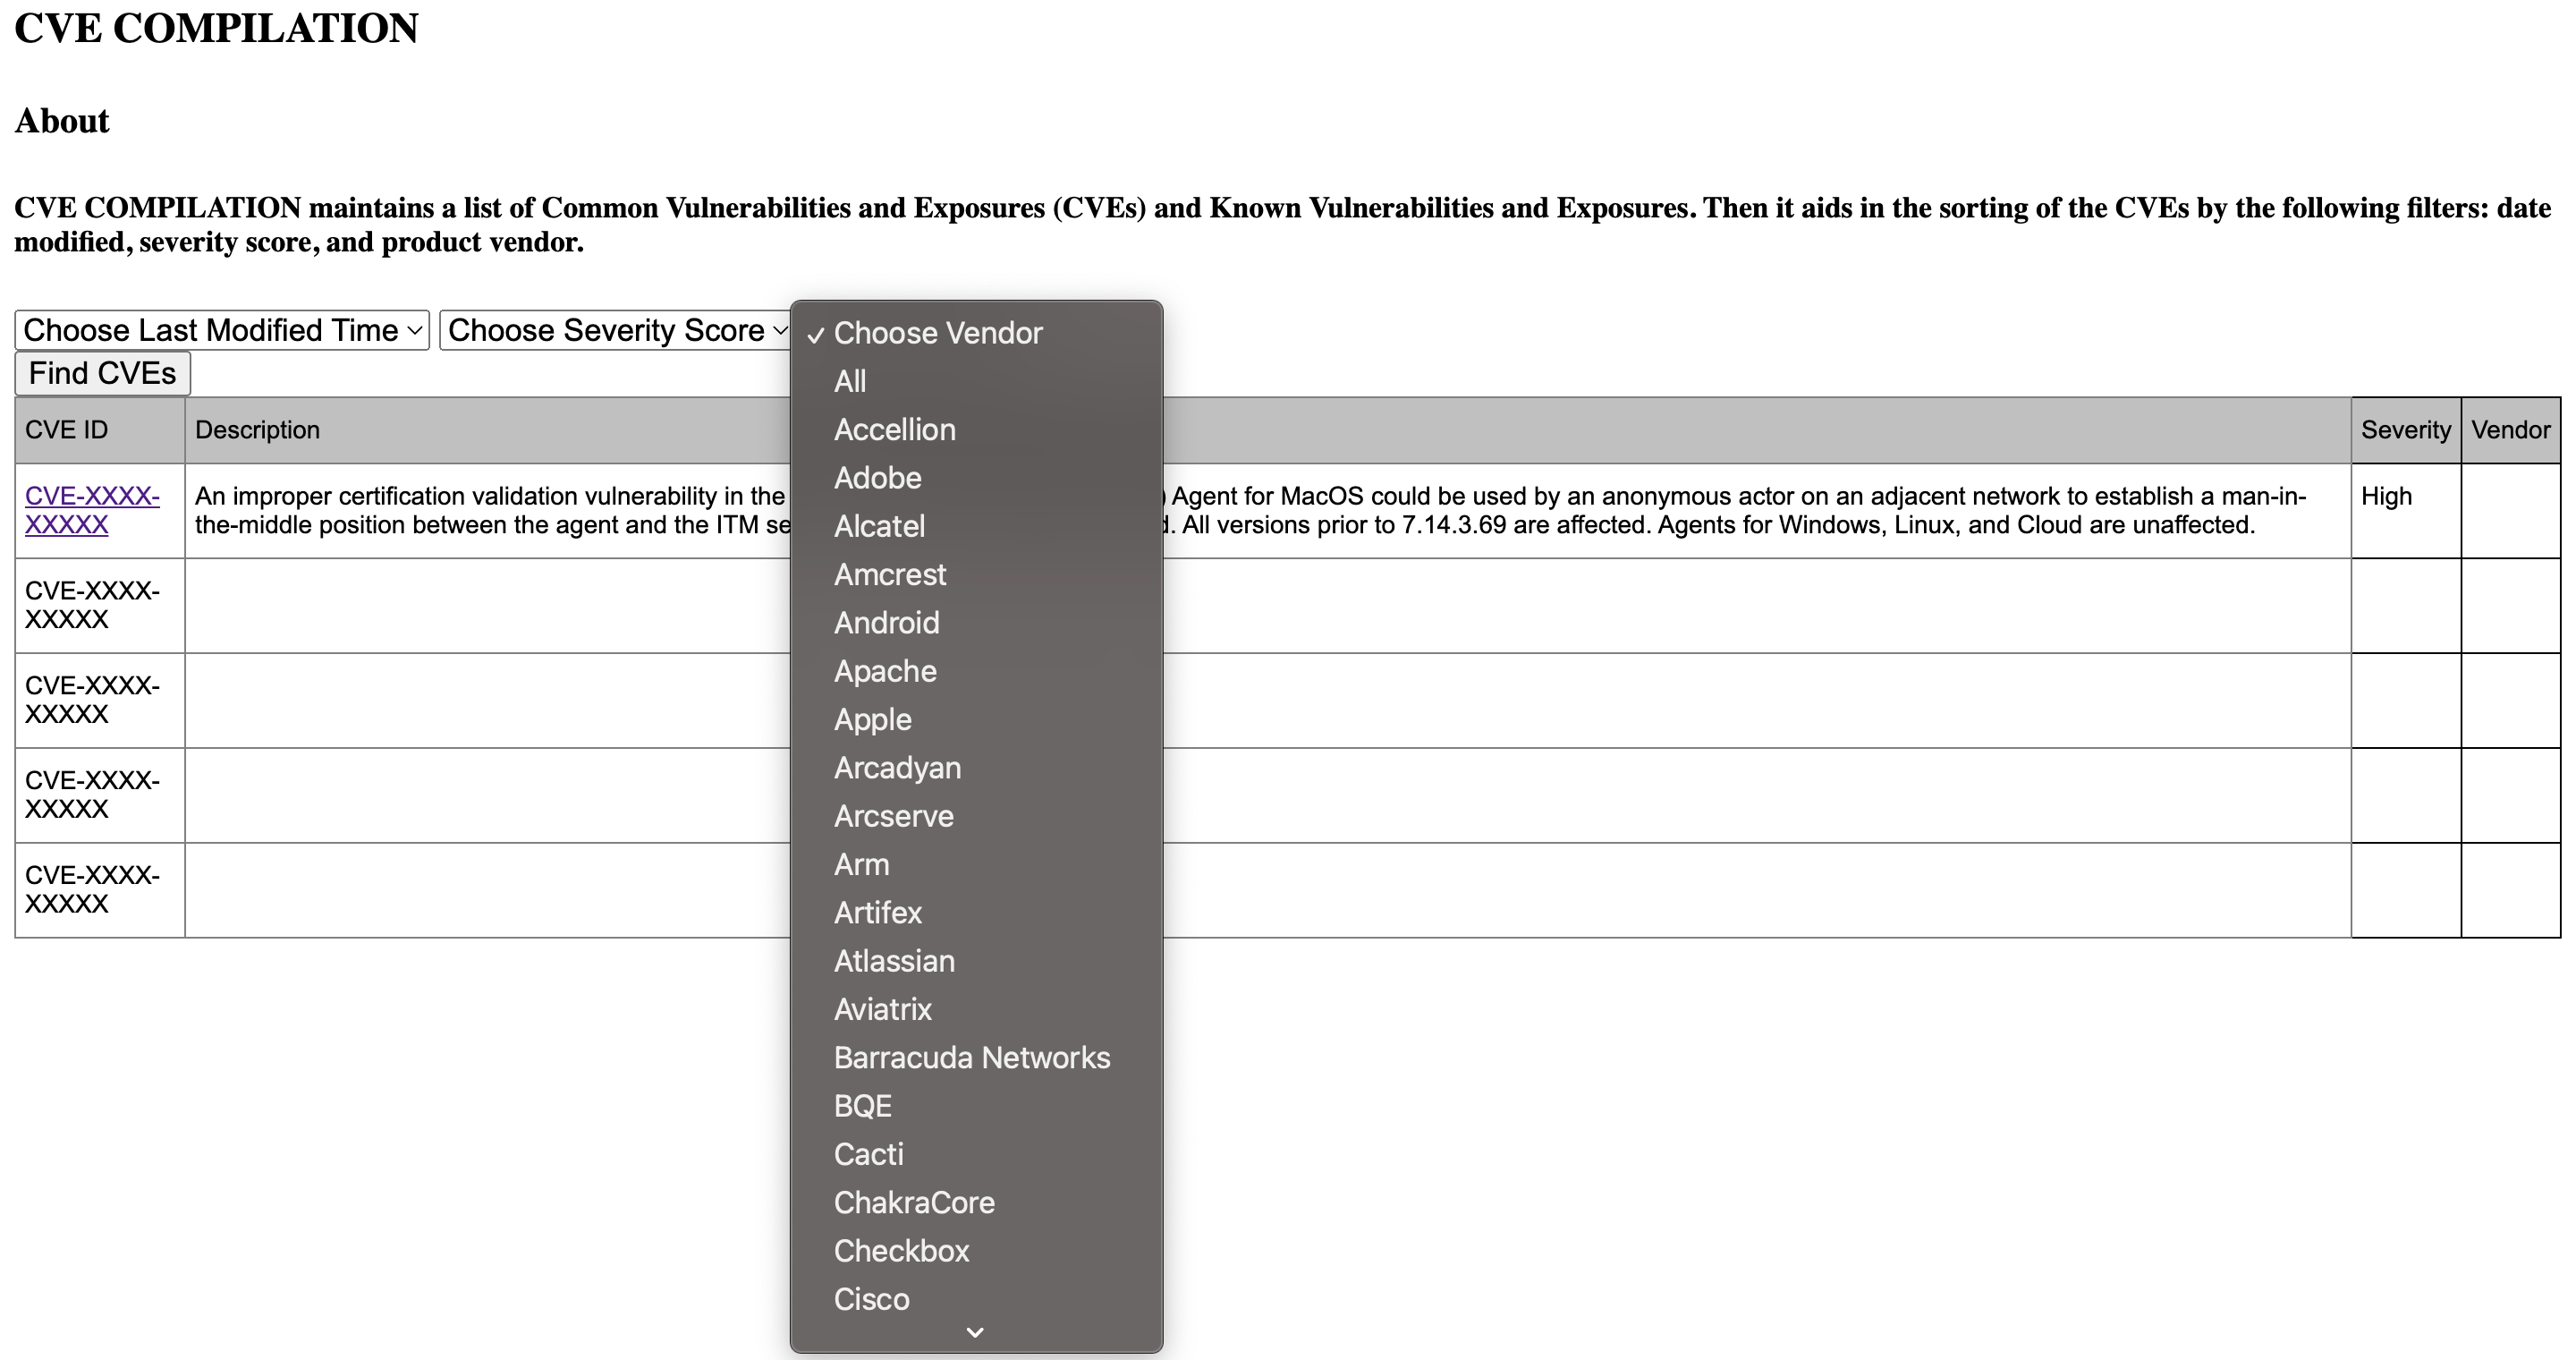
\includegraphics[width=.95\linewidth]{initial-draft.png}
    \caption{
        Initial web application draft with static data.
    }
    \label{fig:initial}
\end{figure}

\subsection{Data Collection}

With an understanding of how I should sort CVEs, I began back-end implementation. The first step was finding the API’s for NIST NVD CVE and CISA. Both of these sites had REST APIs for CVE databases. For both sources, I stored the resulting JSON files separately on my local on my machine since they had extremely different organizations of data within the JSON format. I attempted to combine them, but faced unnecessary difficulty and established that keeping these databases separate provided greater ease for the 'filtering' algorithm step. 

Based on user feedback from my Comps Presentation, I had intentions to update the data using schedule modules in Python. However, my research indicated that this would require the hosting or running of a local machine or server. I also considered including updated datasets in a GitHub repository, however the file sizes were too large to store on GitHub. Eventually, I came up with a more manual solution that gives users some autonomy in the amount of data they want to pull. Users will run one of the following: 

\begin{itemize}
    \item \texttt{update\_data.py} to pull data modified as far back as 1 month
    \item \texttt{update\_data.py -all} to pull data modified as far back as 120 days (Maximum value for NIST NVD CVE database)
\end{itemize}

If they do not currently have \texttt{cve-data-full.json} and \texttt{cisa-data-full.json} files on their local machine, they will now have these. If they already have these files based on previous data pulls, then there are two possible outcomes:

\begin{enumerate}
    \item The data will refresh in these files to ensure it is up-to-date (See Figure \ref{fig:update-data-terminal}). 
    \item The user is informed that their files are already up-to-date. 
\end{enumerate}


While this approach requires an extra step for users, this addressed the question that many of my users had: “How much data does the web application have?” In sum, it is up to the user to decide how much data they would like my web application to filter based on. 

On another note, my databases had nearly complete information, however the NIST NVD CVE database did not include any indication of vendor or product. This is likely because these details are unknown. On the other hand, the CISA database did not have a severity score. There is no obvious explanation for this missing information. But, the CISA database had vendor information because these CVEs have already been successfully exploited somewhere \cite{CISA}. To combat this lack of complete information, my users suggested that I label the CVEs with ‘Unrecognized Vendor’ or ‘Unrecognized Severity’ if there is no available information regarding these ‘filters’.

\subsection{‘Filtering’ Algorithm}
\begin{table}
    \footnotesize
    \begin{tabular}{r|cl}
        \textbf{Filter}       &  \textbf{Preset}    \\
          \hline \\
        Time  &  Today         \\
        Severity Score &  All   \\
        Vendor   &  All         \\
    \end{tabular}
    \caption{Presets for Filters}
    \label{tbl:presets}
\end{table}

The 'filter' defaults were set to 'Today', 'All' and 'All' (See Table \ref{tbl:presets}). These presets were determined in user tests. In early user tests there were no presets and many users decided to click ‘Find CVEs’ without setting all three required ‘filters’. This produced an error. The presets enabled the most convenient search upon initial use of my web application. For instance, in all rounds of user testing, almost all users initially changed ‘vendor’ to match the vendor they were interested in, but they kept the other pre-selections the same. Thus, they only had to adjust one filter before accessing the information that they indicated they most readily needed: today’s vulnerabilities. 

Once a user hits the ‘Find CVEs’ button, the HTTP request collects the selected ‘filter’ variables and sends them to the \texttt{main.py}. I had two ‘filtering' algorithms, one for the NIST NVD data and one for the CISA data. However, the algorithmic components are the exact same, so I will explain the ‘filtering' algorithm once for conciseness (See Figure \ref{fig:flowchart}). The 'filtering' algorithm checks if the CVE publication date ‘matches’ the selected variable for ‘Last Published Time’. If the dates match then the next condition, ‘severity score’, is checked. If the ‘severity score’ of a CVE matches the selected ‘severity score’ filter, then the next condition, ‘vendor’, is checked. If the ‘vendor’ of the CVE matches the selected ‘vendor’ filter, then that CVE and all its contents are added to a dictionary of ‘filtered’ data to be displayed on the web application. If the CVE fails to ‘match’ any of the selected filters then the CVE will not be added to the ‘filtered’ data.

\begin{figure}[ht]
    \centering
    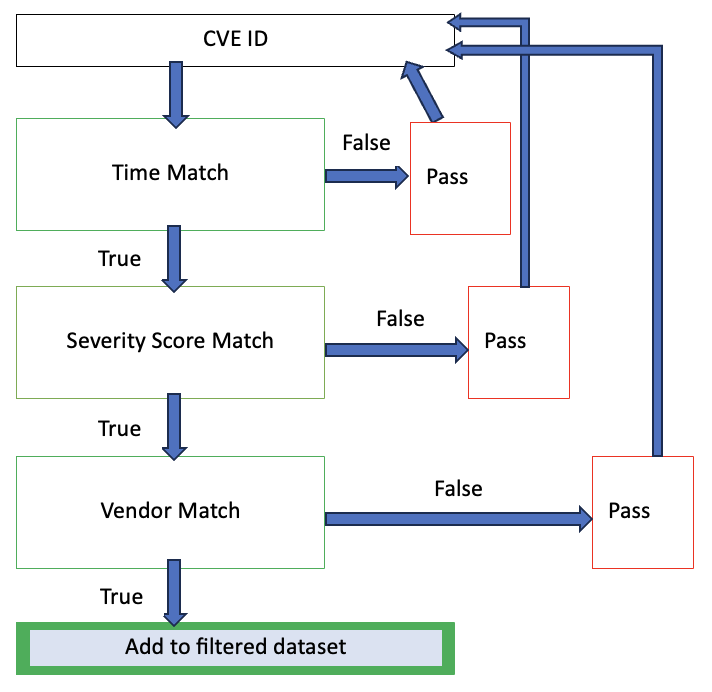
\includegraphics[width=.95\linewidth]{filtering_algorithm.png}
    \caption{
        'Filtering' Algorithm Flowchart.
    }
    \label{fig:flowchart}
\end{figure}

\subsection{Back-End to Front-End}
Once the ‘filtering’ is complete, both ‘filtered’ datasets and the HTML template are passed to Python Flask’s \texttt{render\_template} function. I leveraged Python Flask and used the Jinja2 template to access my ‘filtered’ data and put it in a table format within the HTML file. The choice to display my results in a table (See Figure \ref{fig:full-ui}) was recommended and appreciated by my users as a clear display for the results. Additionally, given the substantial amount of text data I have to display, a table was more effective than visuals like a graph \cite{agostinelli2013data, tukey1990data}. I used JavaScript to implement a loading icon which was recommended by two users since the built-in browser icon was too small to see. Finally, since the functionality of my web application was strong, I dedicated time to ensuring the appearance of my web application enhanced the user satisfaction but did not distract from the functionality. I used CSS to design my HTML to display a ‘dark mode’ aesthetic as opposed to a ‘light mode' since there is some but limited evidence that users experience more satisfaction with ‘dark mode’ since they feel less eye strain \cite{xie2021study}. However, more research suggests that the choice is completely based on user preference \cite{eisfeld2020rise, pedersen2020user}. All of my users appreciated the darker color contrast choices, especially those colors that indicate the differing ‘severity scores’ (See Figure \ref{fig:full-ui}). I call \texttt{render\_template} with the ‘filtered’ data and HTML file as arguments. This produces the final document which serves as the user interface (See Figure \ref{fig:full-ui, fig:no-results, fig:vendor-results}. I did not spend time identifying the order in which I should display the CVE results, because users did not indicate this to be a needed component. 

\begin{figure}[ht]
    \centering
    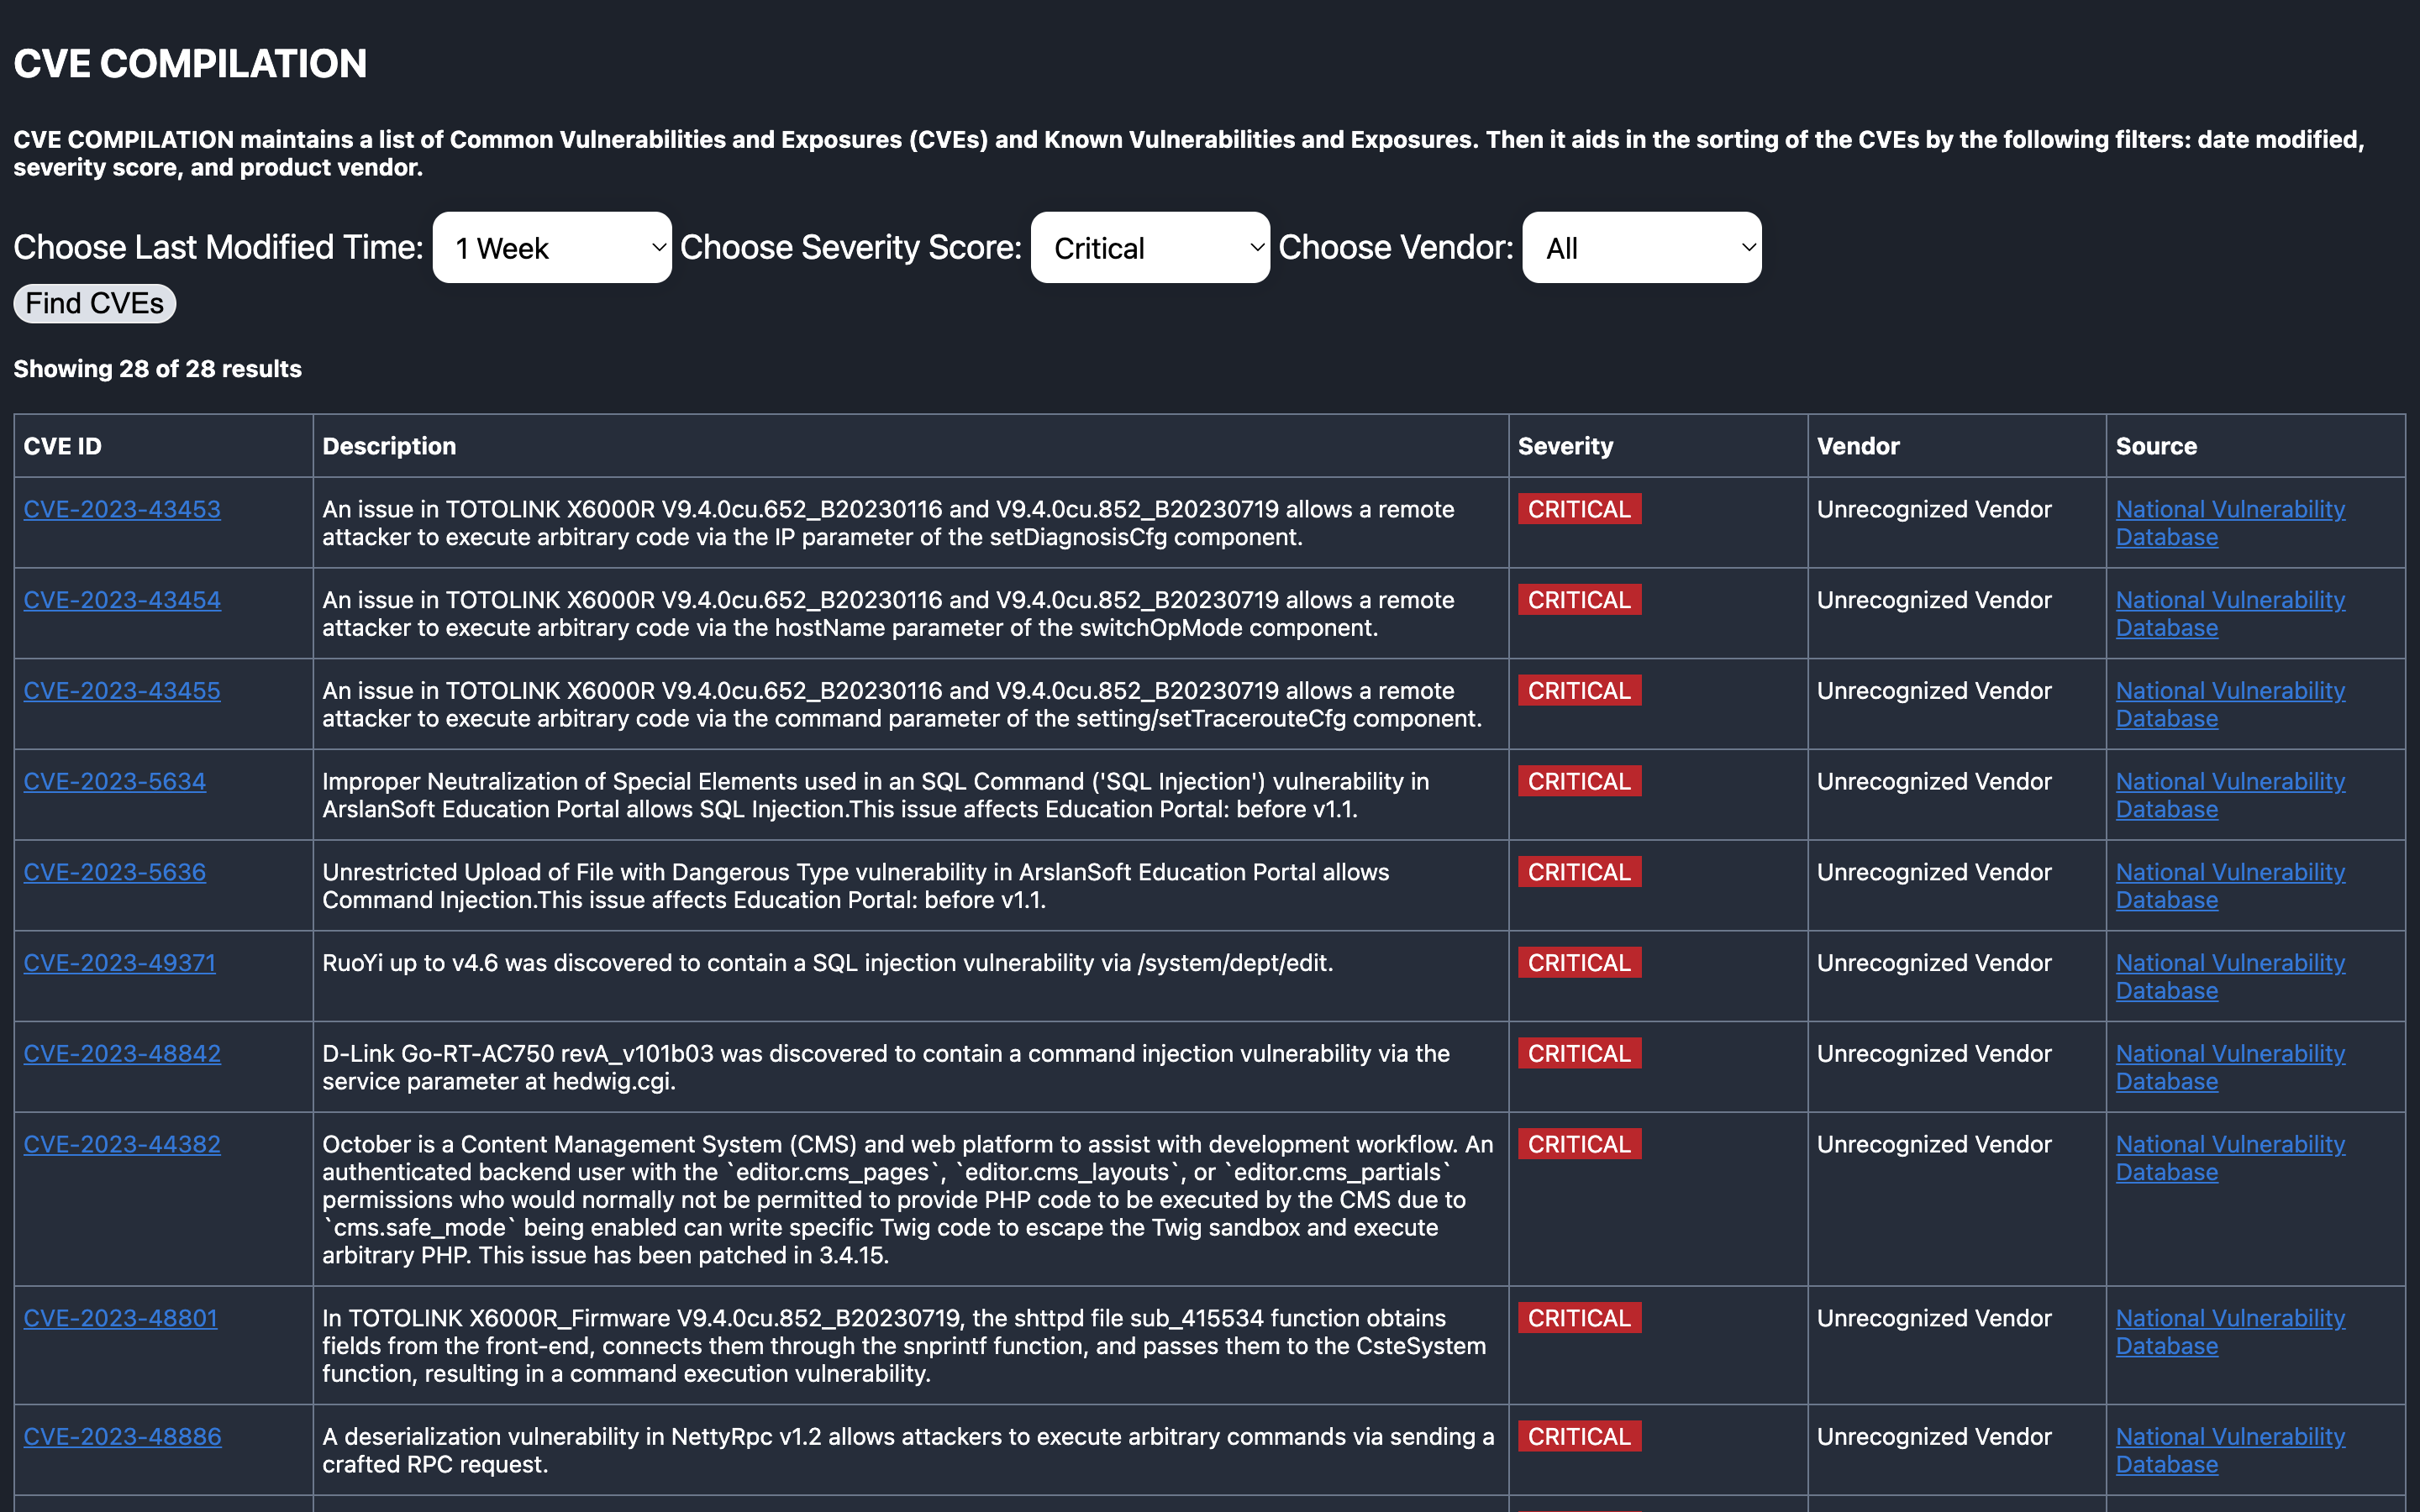
\includegraphics[width=.95\linewidth]{full-user-interface.png}
    \caption{
        Results displayed for CVEs published within the last month, with a critical severity score and any vendor.
    }
    \label{fig:full-ui}
\end{figure}

\begin{figure}[ht]
    \centering
    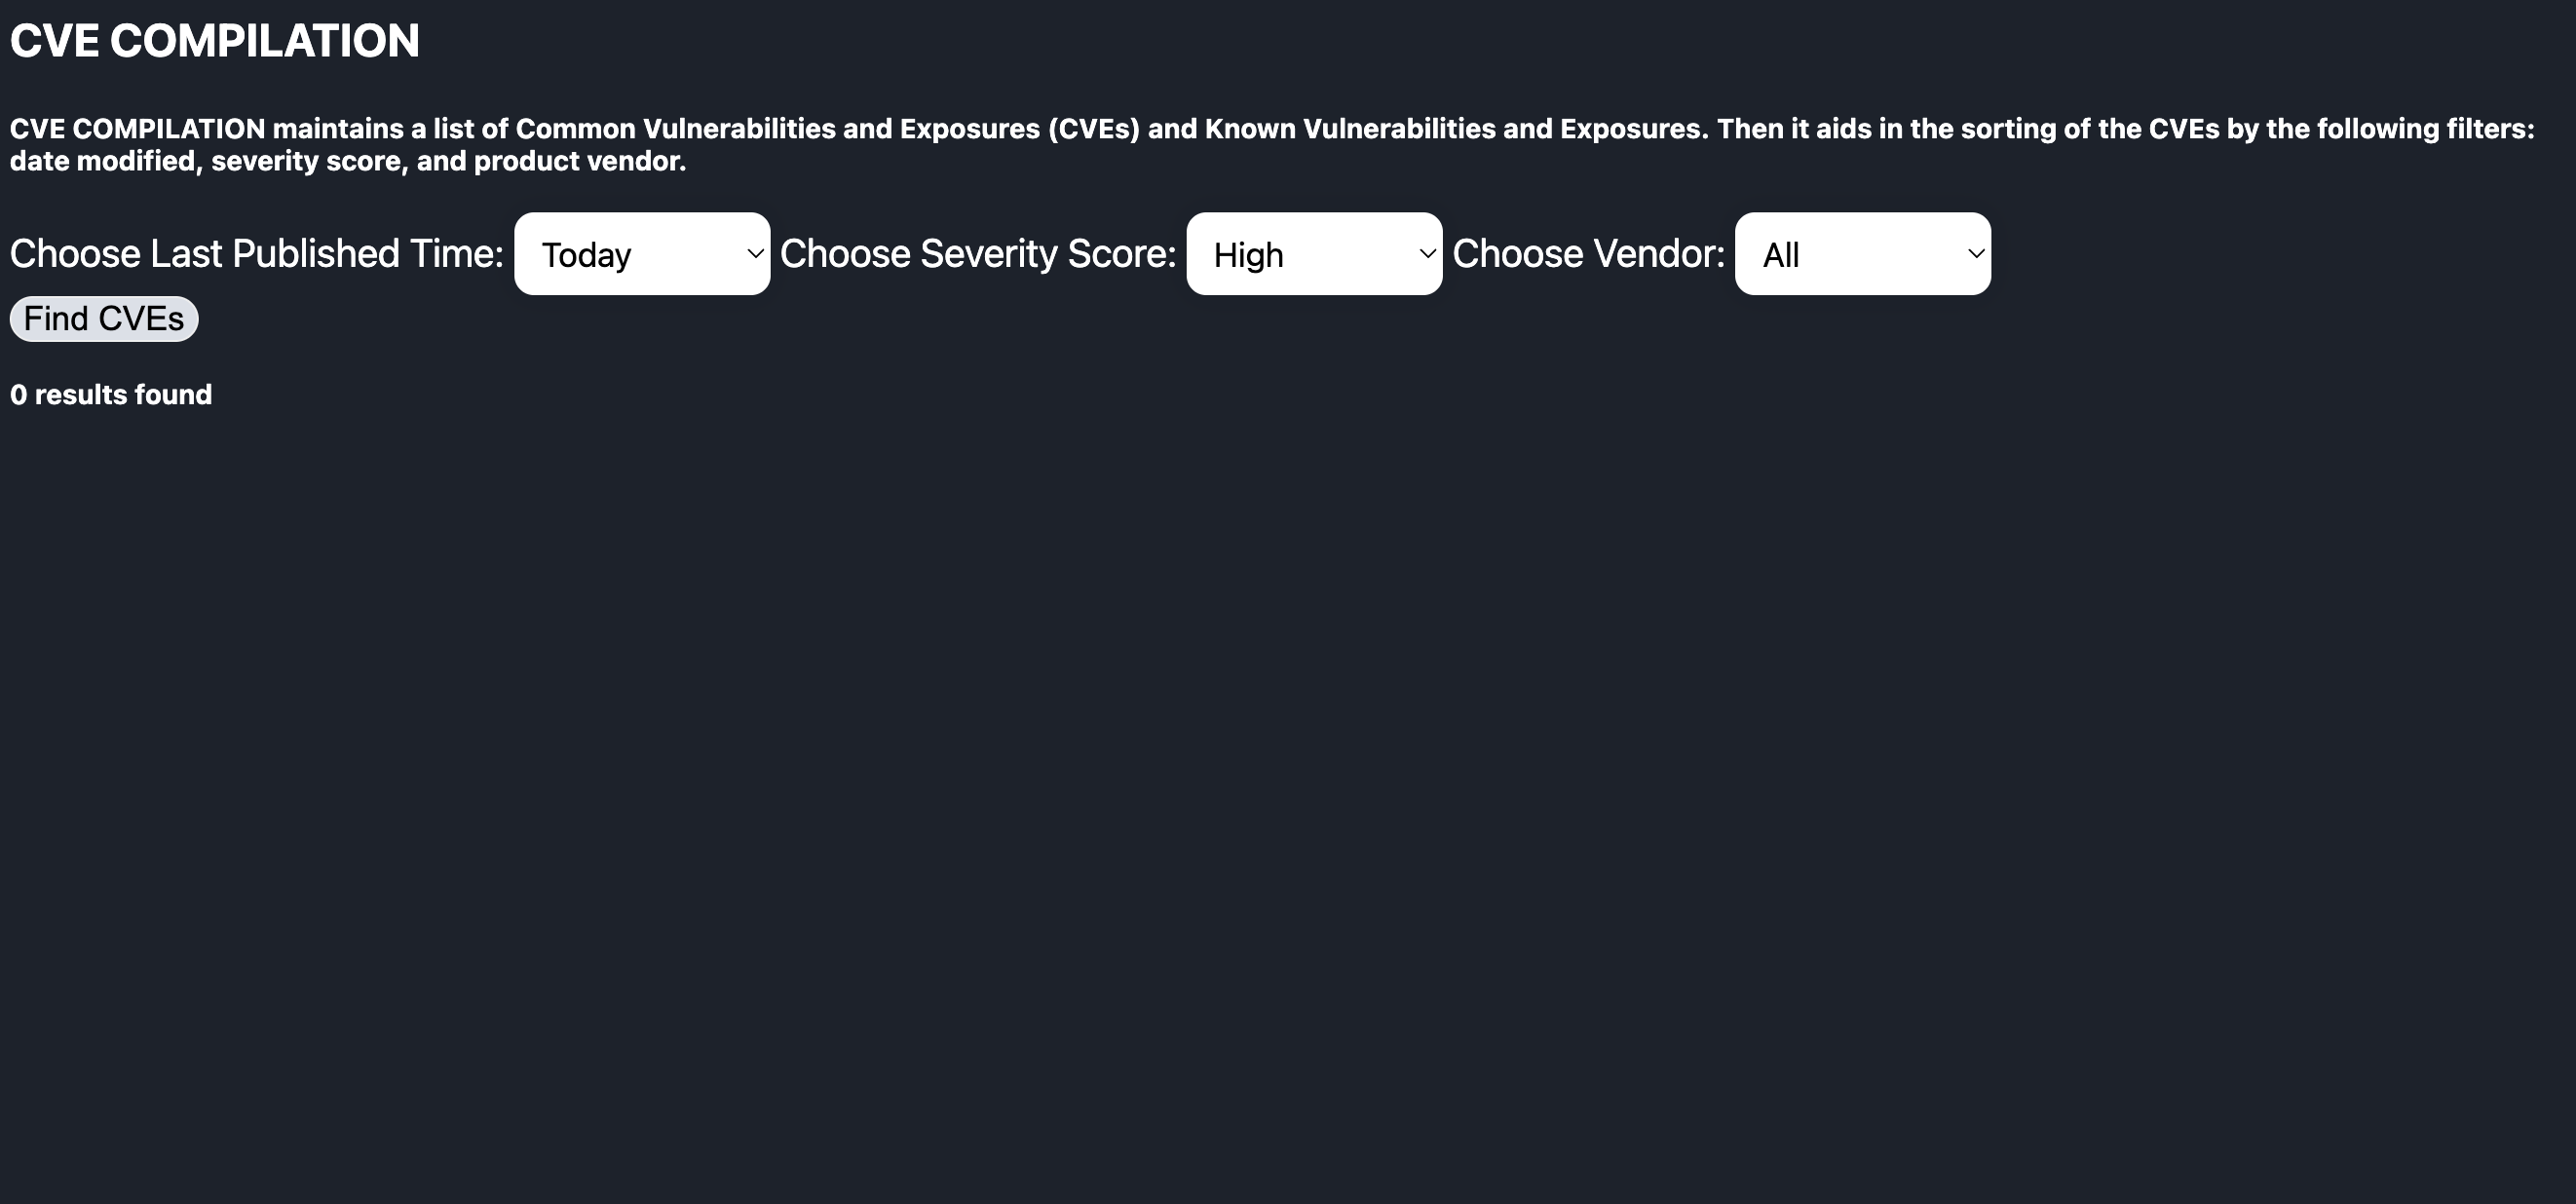
\includegraphics[width=.95\linewidth]{no_results.png}
    \caption{
        No results found for CVEs published today, with a high severity score and any vendor.
    }
    \label{fig:no-results}
\end{figure}

\begin{figure}[ht]
    \centering
    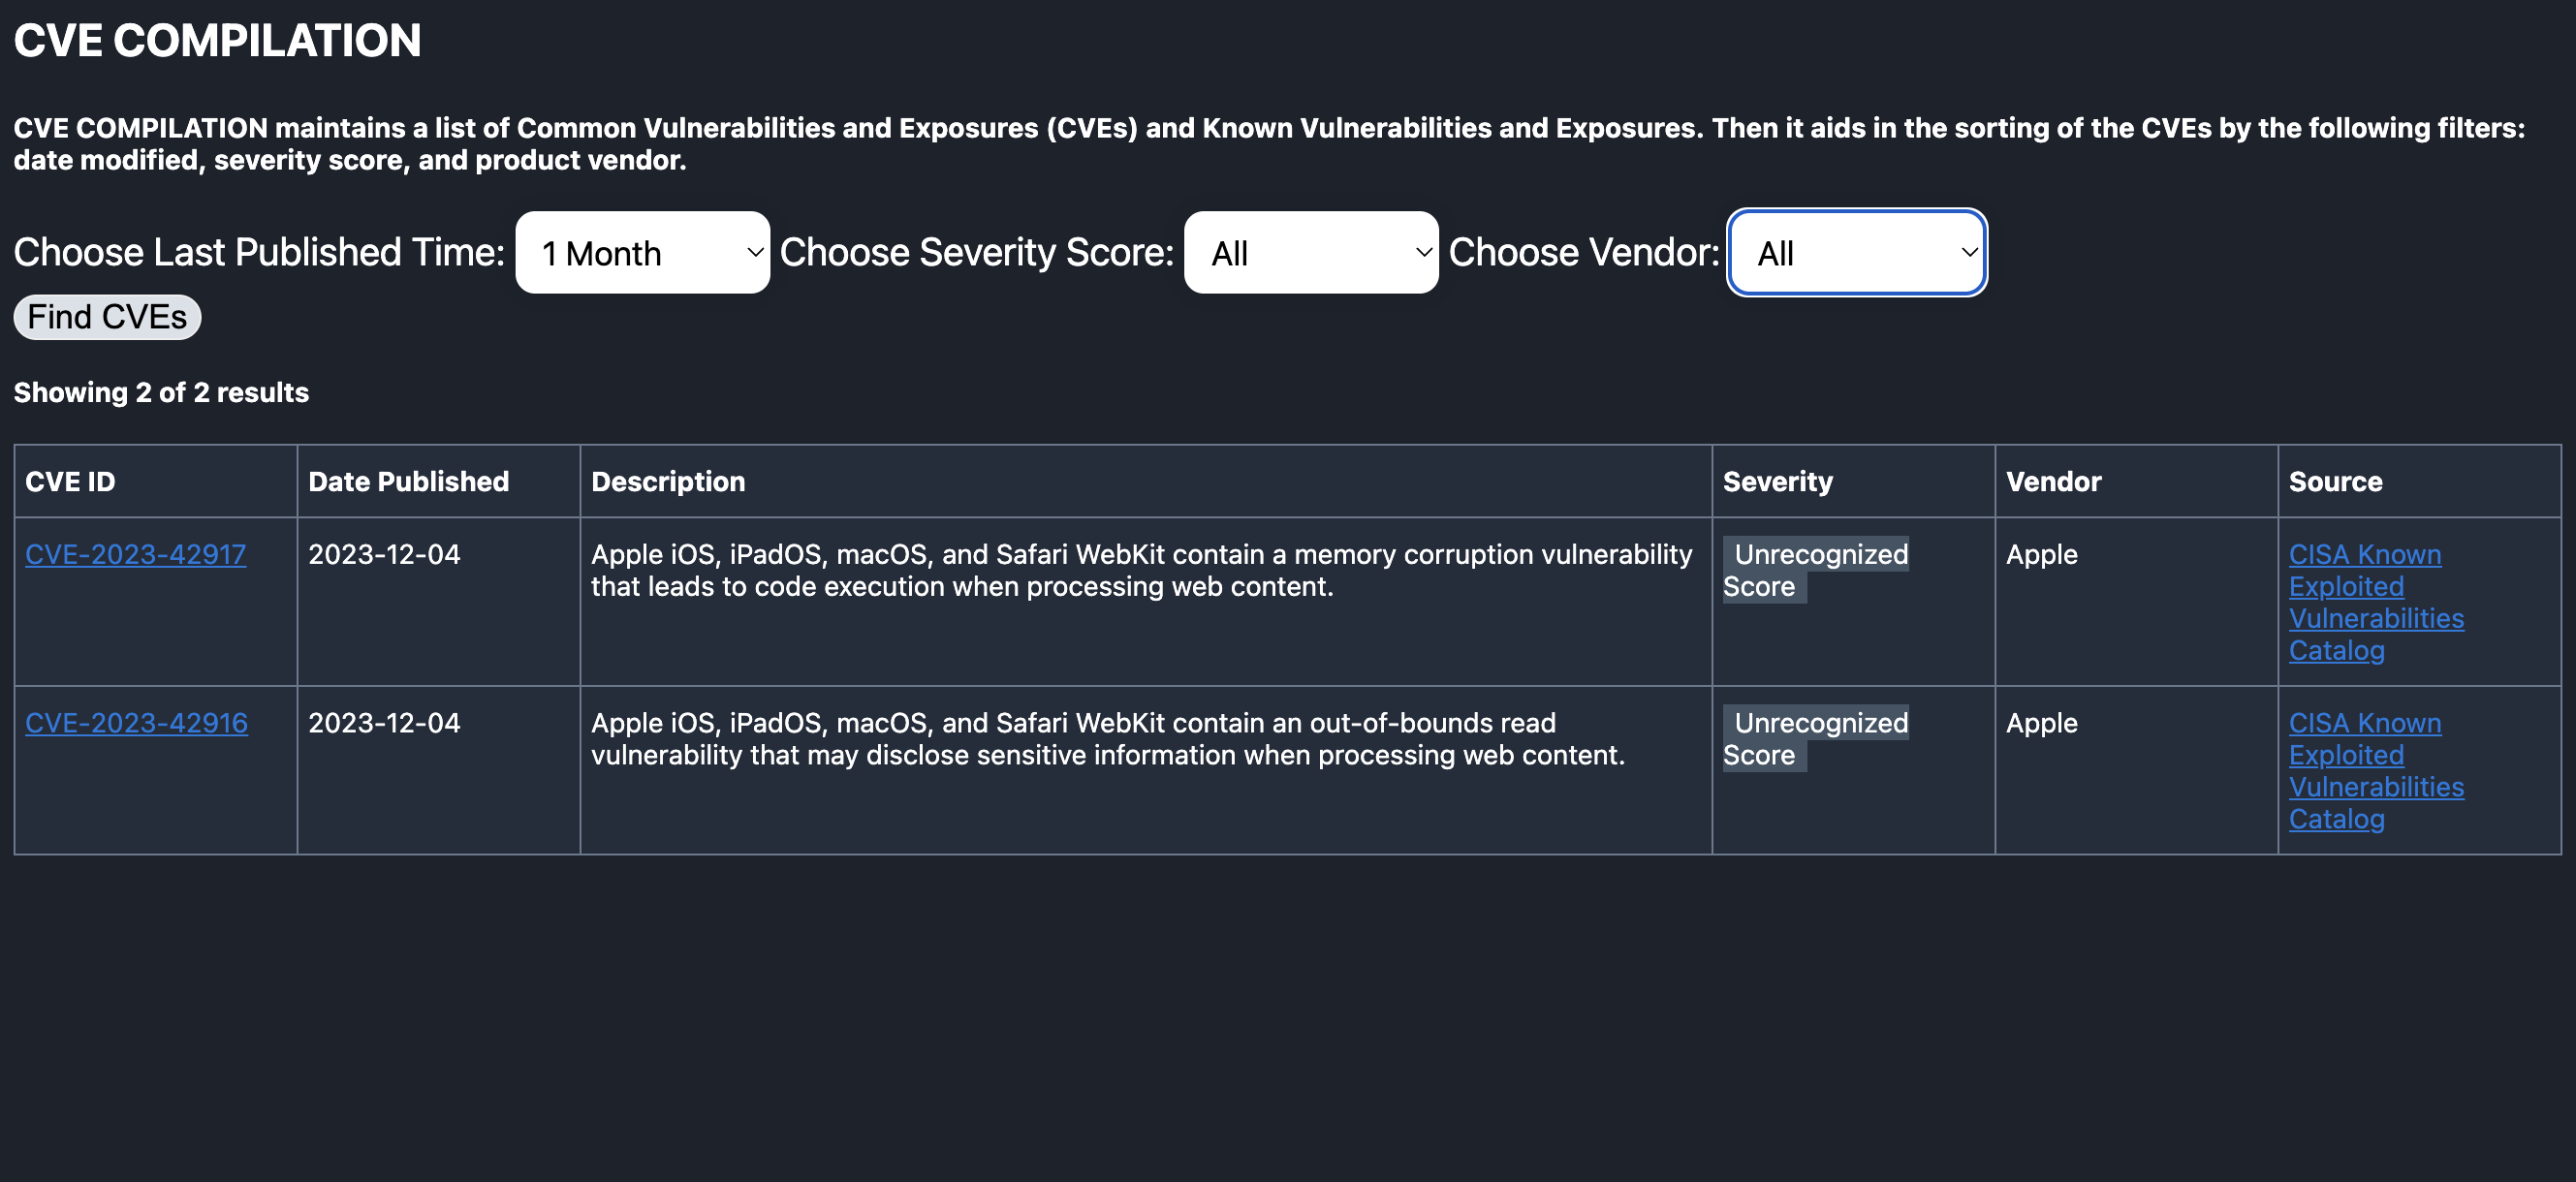
\includegraphics[width=.95\linewidth]{vendor_results.png}
    \caption{
         Results found for CVEs published within the last month, with any severity score and Apple vendor.
    }
    \label{fig:vendor-results}
\end{figure}

\subsection{Final User Tests}  
I have already discussed some results that I collected from user tests (See GitHub for raw data). These user tests involved the user interacting with the web application on my laptop while I watch and take notes. During the final rounds of user-testing, some of the questions I asked based on Dittrich’s \textit{A Beginner’s Guide to Finding User Needs} included: 

\begin{itemize}
 \item Imagine you are no longer getting your email alerts, and this is the  
 \item only site you have access to. Would this fulfill your job needs? Why or why not?
 \item Are there any features you feel like are missing?
 \item Anything else you would like to discuss?
 \item What are you doing with the information that you find on my site?
\end{itemize}

I wanted to support users' decision making once they saw a CVE in my web application. Based on user testing and technical feasibility, providing a link to a page that has patching resources and additional information specific to each CVE in my web application was an effective solution \cite{10.1145/633292.633476}. I address other potential solutions in the future directions section. 

\subsection{User Testing Process} 
For every feature that was brought to my attention in user interviews, I would attempt to implement it before the next round of user testing. During user testing, points of internal conflict came up when I saw the user struggle. I did not know how long I should let the user struggle or produce an invalid result before stepping in \cite{10.1145/633292.633476}. I found that if I had to step in to address the issue after it had been made, that feature needed to be fixed. For instance, when my project took more than four seconds to produce results, users would re-click the ‘Find CVEs’ button thinking that they had not clicked it. I noted that I needed to add a clear loading icon since the default browser one was hard to see and I needed to see if I could increase the efficiency of the search. Now, my project runs so efficiently that the loading icon rarely makes an appearance. 

In my experience, later rounds of user testing were difficult to execute due to the availability of security professionals that I knew in the immediate Los Angeles area. I did not think email communication or video communication was sufficient. As a result, for these later rounds of testing I limited my sample to security professionals at Oxy. 

\section{Evaluation Metrics}
\subsection{Evaluation Methods}
For evaluation methods, I considered controlled A/B tests where two similar populations of users are given different user interfaces, and their responses are measured and compared \cite{rodden2010measuring}. However, due to the tight timeline, I only had time to focus on one version of my project and I also had a small sample size, so splitting the sample into two groups might not have resulted in the most effective measurement. I did not use quantitative metrics such as error counts or task completion times \cite{brooks2010user, spool1996smarter} because I did not have a baseline performance metric, such as time taken to identify daily CVE vulnerabilities through emails, to compare to. Another potential evaluation metric I considered was using a survey, to create an anonymous test of user satisfaction and the usefulness of my web application \cite{rodden2010measuring}. However, I was more interested in watching the user’s interaction with my web application to see how fluidly they navigate the application and what they search for. Additionally, I wanted to encourage users to share their thoughts in real-time so that I could take note. Given the nature of my project, I could interrupt the users to ask questions without disrupting the workflow \cite{spool1996smarter}. As a result, synchronous, in-person user testing was my evaluation method and my evaluation metric was qualitative information. I chose to measure my project based on the HEART metric since it is not focused on one quantitative metric such as the time spent on my web application, but on the whole user experience of my project \cite{flaounas2015evaluation, suryanto2021identifying}. For example, the HEART metric describes user experiences using five key variables \cite{adityo2022user, rodden2010measuring}: 
\begin{enumerate}
    \item Happiness: Do users find the app helpful, fun and easy to use?
    \item Engagement: Do users enjoy application content and want to keep engaging with it? 
    \item Adoption: Do new users see the value in the product or new feature?
    \item Retention: Do users keep coming back to the app to complete a key action?
    \item Task Success: Do users complete their goal quickly and easily? 
\end{enumerate}

For the HEART metric, quantitative metrics are typically employed to evaluate web applications, such as page views, uptime, latency, active users, and monetary earnings \cite{rodden2010measuring}. Since my web application was not publicly accessible or profitable, I altered these common metrics for evaluating so that I could collect metrics during final user tests. Here are the metrics I used to evaluate my project based on the HEART metric: 
\begin{enumerate}
    \item \textbf{Happiness}: Do users find the app helpful, fun and easy to use? 
    \begin{itemize}
        \item \textbf{Metric}: ‘Yes’ or ‘No’
    \end{itemize}
    \item \textbf{Engagement}: Do users seem interested while they are engaging in the web application?
        \begin{itemize}
            \item \textbf{Metric}: Engagement Rating using a five point scale: 1 = Extremely boring; 2 = Boring; 3 = Somewhat engaging; 4 = Engaging; 5= Extremely Engaging.
        \end{itemize}
    \item \textbf{Adoption}: Do users see the value in the product/would they adopt it in their own profession and share it with others in their organization? Why or why not?.
        \begin{itemize}
            \item \textbf{Metric}: ‘Yes’ or ‘No’ and note explanation for further data analysis
        \end{itemize}
    \item \textbf{Retention}: Would users want to use CVE Compilation again in the future? 
        \begin{itemize}
            \item \textbf{Metric}: ‘Yes’ or ‘No’ and note explanation for further data analysis
        \end{itemize}
    \item \textbf{Task success}: Are users able to find the CVE’s that they are looking for and do they discover new ones? 
        \begin{itemize}
            \item \textbf{Metric}: ‘Yes’ or ‘No’ and note any additional comments for further analysis 
        \end{itemize}
\end{enumerate}

The ‘Happiness’ metric was not the main performance related metric, however I wanted to ensure that my web application was not frustrating to use. The ‘Engagement’ metric is necessary to detect if and why the site has enough information to keep them engaged. The ‘Adoption’ and ‘Retention’ metric are different ways of checking the value of my web application for users. Specifically, on initial user interviews, my users indicated that they check for vulnerabilities daily through opening emails particularly from platforms like NIST and CISA. I wanted to measure if the use of my web application removed or decreased the need to check emails for CVEs. This was measured by ‘Task success’.

\subsection{Grading}
For grading, I initially proposed that an A would include a functional NLP analysis of two or more sources with positive user evaluation results and the beginnings of a user interface. And a C would include functional NLP Analysis of two or more sources without positive user evaluation and without a user interface prototype. There have been some alterations to this grading breakdown because I did not have to use any NLP techniques to secure the information that my users wanted present in my web application. Based on this change, an A would include a functional 'filtering' algorithm of two or more sources with positive user evaluation results and the beginnings of a user interface. A C, would include functional filters on two or more sources, but no positive user evaluation results and no have a prototype for a user interface. An F would include no 'filtering' algorithm on two or more sources, thus user testing and a user interface are non-applicable.


\section{Evaluation Results and Discussion}
\subsection{User Evaluation Results}
In the final round of user testing, I performed user evaluations (See GitHub for raw data). For the ‘Happiness’ metric, I received three ‘Yes’ responses and zero ‘No’ responses. For the ‘Engagement’ metric, I received three ‘4’ responses. While I did not receive ‘5’ responses in this category, I am not surprised since this project is not designed to be as engaging as a video game or virtual reality, however the aim is to hold users’ interest while they are searching for CVEs within the web application. For the ‘Adoption’ metric, I received three ‘Yes’ responses and zero ‘No’ responses. I was pleasantly surprised by one of my user’s proposals to deploy the application for others to use. For the ‘Retention’ metric, I received three ‘Yes’ responses and zero ‘No’ responses. Two users noted, “I would definitely use this. This would make my job so much easier.” For the ‘Task Success’ metric, I received three ‘Yes’ responses and zero ‘No’ responses. One user noted the helpfulness of a search feature that could look for keywords in all CVE descriptions and produce the corresponding CVEs. Other users were impressed by the efficiency of the project and ‘dark mode’ appearance. After analyzing my evaluation results, I am most proud of my project’s functionality and adoption rate.

\subsection{Limitations} 
There are several limitations to address. The first is the small sample size of users. I started the project with ten user interviews to discover how cyber security professionals engage with sources of cyber security information. The sample size decreased to five for the first round of user testing and three for the second round of user testing. For the final round of user testing, I was only able to find three cyber security professionals who agreed to participate. The decrease in sample size could be attributed to the fact that I only contacted those who I could meet in-person in the Los Angeles area. For future user testing, I might consider how I could accommodate for asynchronous or remote testing to ensure that I have more users. 
Another limitation is that for the final rounds of my user testing, my sample did not represent a wide range of users. Rather, all users worked for the same organization which calls for a lack of generalizability of my results. The effectiveness of my web application might be attributed to how my users’ organization requires their employees to conduct daily assessments of cyber security threats. Whereas, in other organizations, my web application might not be as effectively incorporated into an employee’s daily workflow. The generalizability remains unclear, however given my initial ten user interviews which included cyber security professionals spanning across five organizations, there was a unanimous need for a centralized platform to access CVEs that were important to the systems that user’s organizations have. Based on the results of my evaluation metrics, my project accomplishes that need. 
Other limitations include the challenging nature of ensuring that user interviews and user testing are as objective and effective as possible. For instance, I strived to create an open environment where the user did most of the talking since I was learning from them. However, in doing this, I found that users would derail from my questions and interview or test goals. I gave them the freedom to share general information and advice as a cyber security professional since I was genuinely interested. However, I found myself breaking up the flow of conversation by redirecting them to questions that I wanted to ask and sometimes I skipped questions or added questions for different users depending on the state of the conversation. Due to these inconsistencies, not all my users experienced the same interview or test process. 

To keep pace with the growing complexity and frequency of cyber attacks, defensive practices are increasingly reliant on proactive measures \cite{behzadan2018corpus}. In regards to defensive practices, my project will help provide information about security vulnerabilities as given by the CVEs. However, it is not likely to reduce the chance of security attacks to occur. Thus, this project should be used as a resource to provide data about CVEs in coordination with other effective cyber security threat patching solutions. For example, my project does not propose how to patch vulnerabilities, but rather it provides a link to possible solutions. Thus, this is not a complete solution for defense against cyber security vulnerabilities, but can only serve as an efficient resource for this solution. 

\section{Ethical Considerations}
\subsection{Web Accessibility}
Since my project is a web app, main ethical concerns include web accessibility which is defined as ensuring navigability and tractability by various users, especially those who have disabilities and face obstacles when interacting with the web \cite{abuaddous2016web}. For instance, people who are blind or who need to use screen reading technology or Braille to access the Web will not be able to access my project \cite{brophy2007web}. Since my web page is compatible with the standard browser users who have visual impairments can zoom in or out as they desire. To access my web page in its current state, there is no need for typing. Thus, those who are physically impaired can access my site by using a mouse or assistive technology such as a joystick.

\subsection{Intended Audience}
Other ethical concerns include socioeconomic variables because my web app requires  consistent access to an electronic device and a strong wireless network connection. Individuals of lower socioeconomic status have less consistent access to computers and high-speed connections compared to individuals of higher socioeconomic status creating an initial gap in my web application’s audience \cite{rothbaum2008parents}. Additionally, my project is designed for an audience of cyber security professionals, or those who have experience in the field of cyber security and understand what CVEs are used for. Individuals not exposed to CVEs will not be able to use or benefit from my web application. My project does not aim to include that audience. If I wanted to include a wider audience, one main feature I would include is educational information on CVEs and their use in the cyber security landscape. 

\subsection{User Decisions}
Another implication is how my users choose to use this information. For instance, if my web application leads a user to ignore a vulnerability because they relied only on the description that my web application provides, then that would be an unintended consequence of my web application. To mitigate the misunderstanding of CVEs or over-reliance on my web application, I also direct them to NIST, a government backed page, which includes further information, such as references to advisories, solutions, and tools, for each specific CVE. In the same vein, my web application could miss a CVE or provide inaccurate information regarding time, severity or vendor. This could result in a negative outcome such as missing a vulnerability to patch or not patching a vulnerability in time. I attempted to mitigate this finding by asking users to identify one of the most recent vulnerabilities they encountered in their other sources and check my web application to see if it was consistent with the one they discovered. Based on this, there were no discrepancies between my web application results and current CVEs, however I think an algorithm would be needed to verify the completeness of my results.  

\subsection{Transparency and Accessibility}
In order to provide full transparency on my project, I will make the source code available via GitHub. The source code of my project will be accessible to anyone for local implementation on their machines if they follow my replication instructions on GitHub. As a result, if there are features that are missing, the code can be maintained and updated by others. This might benefit those who are moderately adept at computer science. In order to decrease this barrier, I provide replication instructions. By making my source code accessible, I hope that I can serve as a rudimentary resource for cyber security experts at small organizations who are interested in quickly finding out about relevant and current CVEs without needing to allocate significant financial resources to this task. There is research that indicates the unruly costs of cyber security controls and defensive practices \cite{kesswani2015maintaining, CIS}.

\section{Future Work and Conclusion}
\subsection{Future Work}
Future work includes expanding upon this project to include other helpful features such as a search box that identifies keywords in CVE descriptions. Other features that I am unsure of how to implement include identifying product version numbers. With this information I would filter by version numbers and display version numbers in my CVE table of results. Furthermore, future work could explore how to include patching solutions guidelines or tutorials for every CVE to assist cyber security professionals patch vulnerabilities on their specific systems. This would require some level of customization and I could imagine this would be more of an educational and assistive feature particularly benefiting organizations that have less resources to devote to cyber security. 

\subsection{Conclusion}
In conclusion, I began this project by identifying a common problem amongst cyber security professionals: combing through emails or commonly used cyber security news sites to identify what CVEs are relevant to an individual’s systems and which ones needed patching was not an effective use of time or cyber security resources. I conducted user tests to identify what features my web application should include to expedite or solve this problem. In between user tests, I implemented new features and made changes to existing ones for the next round of user testing. I successfully completed a web application that includes filtering of CVEs by time added, severity score and vendor as well as links to pages that contain official solutions and patches. Feedback from user evaluations suggested that my web application is a resource used among cyber security professionals to streamline their daily search and patching tasks for vulnerabilities and exposures.


\section{Replication Instructions}
\begin{enumerate}
    \item Install Python
    \begin{enumerate}
        \item Download \href{https://www.python.org/downloads/}{Python}. Any version later than 3.8.5 is acceptable
    \end{enumerate}

    \item Create Virtual Environment
    \begin{enumerate}
    \item Create a project folder and a \texttt{.venv} folder within. Type the following terminal commands: 
        \\ \texttt{\$ mkdir Project}
        \\ \texttt{\$ cd Project}
        \\ \texttt{\$ python3 -m venv .venv}
    \end{enumerate}

    \item Activate the Environment
        \begin{enumerate}
        \item Activate the corresponding environment before you work on your project
        \end{enumerate}

    \item Install Python Flask
    \begin{enumerate}
        \item Within the activated environment, type the following command to install \href{https://flask.palletsprojects.com/en/3.0.x/installation/}{Flask}
        \\ \texttt{\$ pip install Flask}
    \end{enumerate}

    \item Install Requests
    \begin{enumerate}
        \item Within the activated environment, use the following command to install the \href{https://pypi.org/project/requests/}{Requests HTTP library}
        \\ \texttt{\$ pip install requests}
        Or 
        \ \texttt{\$ python -m pip install requests}
        \item To upgrade requests to the latest version, type the following command: 
	\\ \texttt{\$ pip install --upgrade requests}
    \end{enumerate}

    \item Cloning the GitHub Repository
    \begin{enumerate}
        \item In the terminal or command prompt navigate to the Project folder you just created. Type the following command: 
	\\ \texttt{\$ cd Project}
        \\\item Clone the Git repository. Type the following command:
        \\ \texttt{\$ git clone https://github.com/e-corwin/
        \\ security-vulnerability-webapp.git}
    \end{enumerate}

    \item Requesting API Keys
    \begin{enumerate}
        \item In order to retrieve data from the NIST NVD CVE database, you need an API key. Request from the following \href{https://nvd.nist.gov/developers/request-an-api-key}{form}. 
        \item Create a new file called \texttt{key\_variable.py}. Include the following line of code with your API key in this file:
        \ texttt{Headers = \{'apiKey': 'insert API Key here'\}}
    \end{enumerate}

    \item Opening the Repository on Your Local Machine
        \begin{enumerate}
            \item Open the files in VSCode or an IDE or code editor of your choice. 
        \end{enumerate}

    \item Loading the Dataset
        \begin{enumerate}
            \item Run \texttt{update\_data.py} to pull CVE data modified within the last month. If you want to pull CVE data modified within the last 120 days, run: 
            \texttt{\$python update\_data.py -all}. 
            You should see the following: 
\begin{figure}[ht]
    \centering
    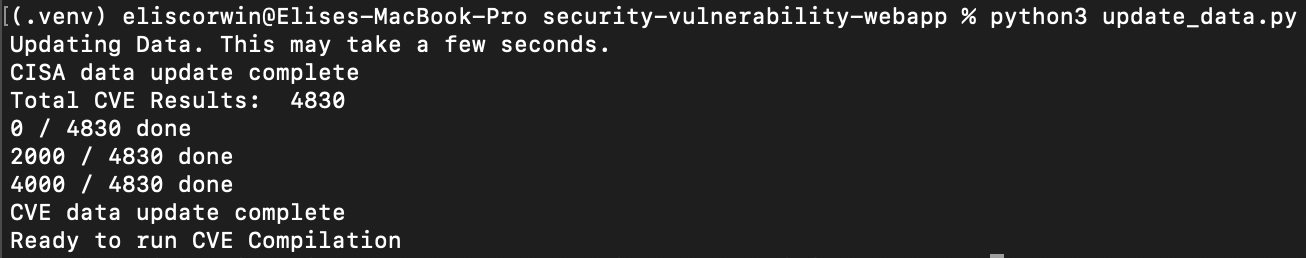
\includegraphics[width=.95\linewidth]{update_data_terminal.png}
    \caption{
        Terminal after \texttt{update\_data.py}.
}
    \label{fig:update-data-terminal}
\end{figure}
        \end{enumerate}

Note that the number of results will likely be different from what is shown here. If this is your first time loading the dataset, new files \texttt{cve-data-full.json} and \texttt{cisa-data-full.json} will be created and populated with data. If this is not your first time loading the dataset, \texttt{cve-data-full.json} and \texttt{cisa-data-full.json} will be updated. 

    \item Running the Web Application
        \begin{enumerate}
            \item Run \texttt{main.py}
            You should see the following:
    \begin{figure}[ht]
    \centering
    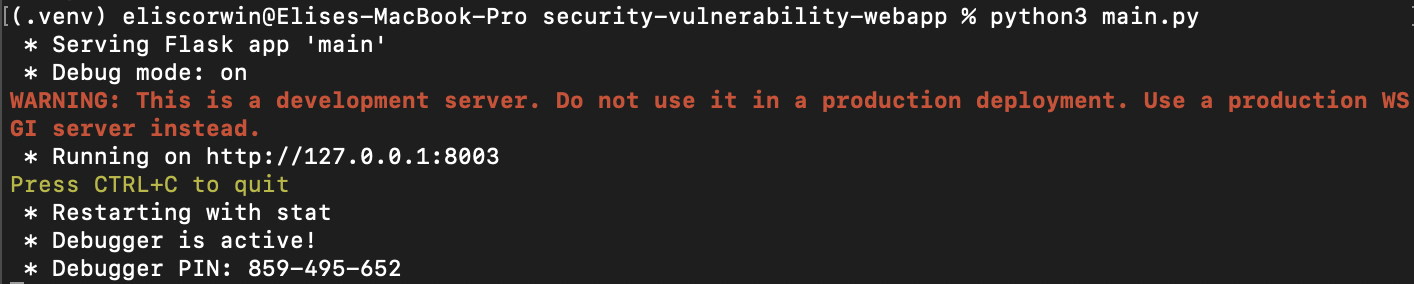
\includegraphics[width=.95\linewidth]{app_run_terminal.png}
    \caption{
        Terminal after running \texttt{main.py}.
    }
    \label{fig:app-run-terminal}
\end{figure}

            \item Paste the server the app is running on in a browser. I used Google Chrome. You should now see the Web application. 
        \end{enumerate}
\end{enumerate}

\section{Code Architecture Overview}
For a visual interpretation of the code see Figure \ref{fig:code-architecture}. Data is pulled from the NIST NVD API and the CISA API and stored in JSON files. The 'filtering' algorithm receives 'filter' input from the \texttt{main.py} file and executes to produce the 'filtered' data. The HTML and CSS files access the 'filtered' data passed by the main template to produce the document for the CVE Compilation web application. 

\begin{figure}[ht]
    \centering
    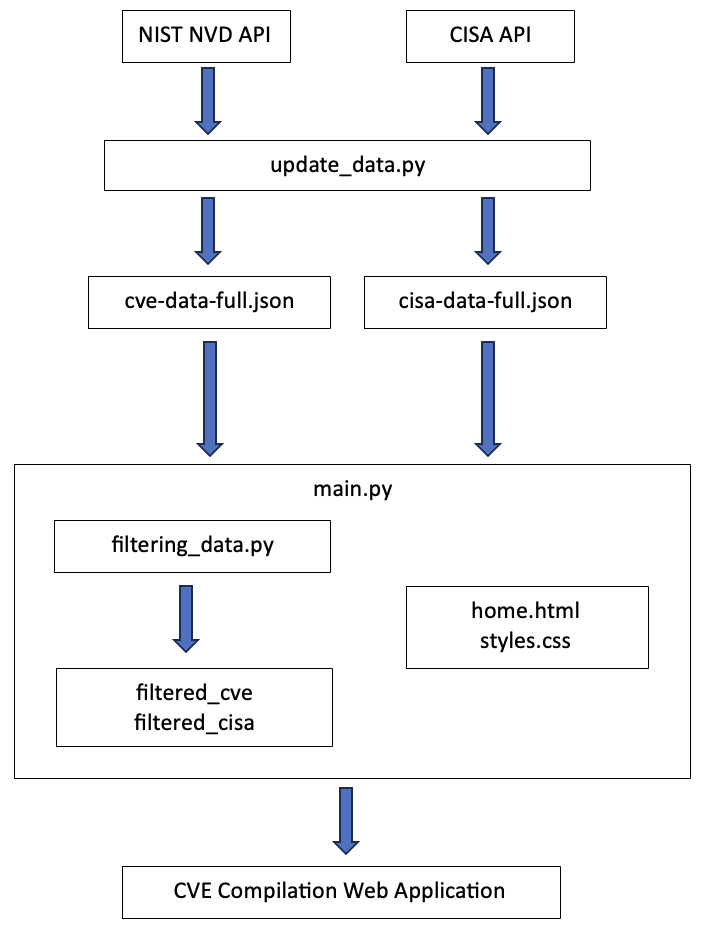
\includegraphics[width=.95\linewidth]{code_architecture.png}
    \caption{
        Code Architecture Overview
    }
    \label{fig:code-architecture}
\end{figure}

\printbibliography

\end{document}
